\documentclass[12pt]{article}% 这是主要的格式。
\usepackage[UTF8]{ctex}
\usepackage[page,title,titletoc,header]{appendix} 
\usepackage{enumerate}
\usepackage{amsmath}
\usepackage{graphicx}
\usepackage[labelsep=space]{caption}
\usepackage{cite}
\usepackage{textcomp}
\usepackage{array}
\usepackage{bigstrut}
\usepackage{geometry}
\usepackage{graphicx}  
\usepackage{subcaption}
\usepackage{xcolor}  
\usepackage{listings}  
\usepackage{color}  
\usepackage[framed,numbered,autolinebreaks,useliterate]{mcode}
\geometry{left =2.5 cm,right=2.5cm,top=2.5cm,bottom=2.5cm}
\usepackage[section]{placeins}
\usepackage[colorlinks,linkcolor=black,citecolor=black]{hyperref}
\usepackage{titlesec}  
\usepackage{titletoc}
\usepackage[framed,numbered,autolinebreaks,useliterate]{mcode}
\titleformat{\section}{\centering\heiti\zihao{4}}{\thesection}{0.3em}{}
\titleformat{\subsection}{\heiti \fontsize{12pt}{0}}{\thesubsection}{0.3em}{}
\titleformat{\subsubsection}{\heiti \fontsize{12pt}{0}}{\thesubsubsection}{0.3em}{}
\renewcommand\figurename{\heiti\zihao{5} 图}
\renewcommand\tablename{\heiti\zihao{5} 表}


\title{ \heiti\zihao{3}基于的诺基亚香蕉机评估}
\author{}
\date{}

\begin{document}
\pagenumbering{Roman}
\tableofcontents
\newpage
\pagenumbering{arabic}
\setcounter{page}{1}
\section{问题重述}
\subsection{问题的背景}
随着科技的发展,智能手机已经成为多数人生活中必不可少之物。而曾经是手机行业翘楚的诺基亚一度因为对市场的误判消失在大众视野中,但是,诺基亚在悄悄回归。在MWC 2018大展上,诺基亚正式宣布了8110经典机型的复刻计划,机身采用弧形波浪的时尚设计。在营销中,主推黄色,被昵称为“香蕉机”,较受瞩目和追捧。

而在硬件配置上,诺基亚8110是一部搭载2.4英寸QVGA彩色屏幕和200万像素后置摄像头的手机,支持双卡和LTE连接,功能机OS内置应用商店和新版贪食蛇游戏,最长待机时间可达25天。新的4G复刻版依然是下滑盖,机身更薄,携带方便。名为复古,实际上做了重新设计,屏幕更大、调整键盘布局,支持4G LTE,内置地图、流行社交软件等应用。该款手机目前开始在亚洲上市销售,售价远低于流行的智能手机。

任何一种新产品投放市场,各种变化与不确定性都将检验其投放市场前的预判,需要根据实际市场反馈和企业未来发展进行调整。

根据上述背景,请回答以下问题。

\subsection{需要解决的问题}
\begin{enumerate}[(1).]\addtolength{\itemsep}{-1.5ex}
\item 试从企业的产品设计、生产制造、营销、测试、维护、研发、安全等环节,建立数学模型,说明企业如何管理来实现利润最大化。
\item 针对诺基亚推出的Nokia 8110香蕉机,适当减弱了娱乐功能,强调实用功能,其预设购买对象为怀旧、注重设计感、学生等人群。经过一段时间销售后,调查分析实际购买人群与预设人群是否存在差异,优化问题(1)中的模型,使得企业的利润获取最大。
\item 作为诺基亚公司董事会的一名高层管理者,请写出一份(不超过两页)新推Nokia 8110香蕉机的全面评估报告,强化向社会融资和银行贷款的信心。
\end{enumerate}
\section{问题分析}
\subsection{问题的重要性分析}
对于现今社会而言,智能手机已成为人们必不可少的物品,作为诺基亚重新获得智能手机市场的重要一步,Nokia 8110香蕉机无疑成为关键的一棋。

同时,任何一种新产品-自然也包括诺基亚Nokia 8110香蕉机-投放市场,各种变化与不确定性都将检验其投放市场前的预判。

因此如何根据实际市场反馈和企业未来发展来调整相应的营销方案,以及如何做到利润最大化,都是需要解决的问题。

\subsection{文献综述}
许茂增,唐飞考虑了消费者对新产品、再制造产品和二手产品的偏好程度不同,建立了闭环供应链差别定价模型,研究了制造商是否从事再制造和经销商是否经销二手产品的生产决策问题\cite{xu}张旭梅,官子力等则考虑了电信服务具有的网络外部性,基于效用理论,建立手机制造商和电信运营商的利润函数\cite{zhao}。翁世淳,黄维则将连锁店悖论模型和KMRW声誉模型结合起来,构建适合分析非合作博弈下智能手机定价策略来得到相应的结果\cite{weng}。

但大多数同类型的文献,是以后期投放市场后的情况来作为依据,而缺少对于产品的先验性分析。
\subsection{问题的思路分析}
\begin{enumerate}[1.]\addtolength{\itemsep}{-1.5ex}
\item 针对问题一,需要从7个环节的投入情况和最终收益情况来考量,得到利润与各个环节投入情况的关系,来得到企业的利润最大化条件。
\item 针对问题二,需要考虑实际购买人群的差异所导致的企业利润变化,对问题一的模型进行一定的优化。
\item 针对问题三,需要结合问题二的结果,对Nokia8110的相关现状作具体分析,确认其是否满足利润最大化的条件。
\end{enumerate}
\section{问题假设}
为了简化模型,同时更好地进行分析,我们做出如下假设:
\begin{enumerate}[1.]\addtolength{\itemsep}{-1.5ex}
\item假设所有获得的数据真实可靠;
\item假设各个环节的投入资金是不相关且独立的,即某一环节投入的资金增加,只影响最终利润,而不影响之前或之后环节的资金投入;
\item 假设产品设计、生产制造、营销、测试、维护、研发、安全等7个环节对最终利润均有影响,且影响足够大,即单独改变某一环节的资金投入,能够对利润产生影响;
\item 假设各环节对影响是可量化的,即对于确定的投入情况,应当可以得到确定的利润;
\item 假设各环节均不作任何投入时,没有利润。
\end{enumerate}
\section{符号说明}
\begin{table}[htbp]
  \centering
    \begin{tabular}{cc}
    \hline
    符号 & 解释说明 \\
      \hline
   $ x_1$ & 产品设计投入 \\
    $x_2$ & 生产制造投入 \\
    $x_3$ & 营销投入 \\
    $x_4$ & 测试 投入\\
    $x_5$ & 维护投入 \\
    $x_6 $& 研发投入 \\
    $x_7 $& 安全 投入\\
    $y $ & 利润 \\
         \hline
    \end{tabular}%
  \label{tab:addlabel}%
\end{table}%
\section{模型的建立及求解}
\subsection{模型一:基于多项式回归的利润最大化模型}
\subsubsection{模型的准备}
针对问题一,我们首先要搜集各环节投入的资金与利润情况,借助多元非线性回归,得到
根据可查询到的各公司的财务报表的相关数据,整理得到关于苹果公司\cite{pingguo}、中兴公司\cite{zhongxing}、小米公司\cite{xiaomi}的相关情况,见表\ref{tab:addlabel11}-\ref{tab:addlabel31}。

其中生产制造费用期末结转到生产成本,因此结转后的生产制造费用不会在财务报表体现。而生产成本则在资产负债表中以存货的方式反映,这里以存货近似代替生产制造费用。

由于单位存在一定差异,为统一单位,将表\ref{tab:addlabel11}做一定处理,截至2018年7月4日0时,人民币对美元汇率为6.6368,由此,得到表\ref{tab:addlabel41}及最终学习数据集表\ref{tab:addlabel55}。

\begin{table}[htbp]
  \centering
  \caption{苹果公司利润与各环节投入间关系情况表\\单位:百万美元}
    \begin{tabular}{ccccccccc}
    \hline
    时间 & 产品设计 & 生产制造 & 营销 & 测试 & 维护 & 研发 & 安全 & 利润 \\
        \hline
    2007 & 1832 & 346 & 15852 & 374 & 2963 & 782 & 323 & 3496 \\
    2008 & 2455 & 509 & 21334 & 487 & 3761 & 1109 & 365 & 4834 \\
    2009 & 2954 & 455 & 25683 & 548 & 4149 & 1333 & 370 & 8235 \\
    2010 & 4768 & 1051 & 39541 & 729 & 5517 & 1782 & 343 & 14013 \\
    2011 & 7777 & 776 & 64431 & 1002 & 7599 & 2429 & 323 & 25922 \\
    2012 & 15452 & 791 & 87846 & 1342 & 10040 & 3381 & 336 & 41733 \\
    2013 & 16597 & 1764 & 106606 & 1530 & 10830 & 4475 & 403 & 37037 \\
    2014 & 20624 & 2111 & 112258 & 1803 & 11993 & 6041 & 432 & 39510 \\
        \hline
    \end{tabular}%
  \label{tab:addlabel11}%
\end{table}%

\begin{table}[htbp]
  \centering
  \caption{中兴公司利润与各环节投入间关系情况表\\单位:百万人民币}
    \begin{tabular}{ccccccccc}
      \hline
    时间 & 产品设计 & 生产制造 & 营销 & 测试 & 维护 & 研发 & 安全 & 利润 \\
      \hline
    2012 & 1429 & 1799 & 6347 & 1550 & 12485 & 3130 & 1468 & -813 \\
    2013 & 1839 & 1144 & 7295 & 1256 & 10150 & 2550 & 1293 & 2879 \\
    2014 & 1600 & 1243 & 6097 & 1144 & 10052 & 2382 & 1051 & 1950 \\
      \hline
    \end{tabular}%
  \label{tab:addlabel21}%
\end{table}%
\begin{table}[htbp]
  \centering
  \caption{小米公司利润与各环节投入间关系情况表\\单位:百万人民币}
    \begin{tabular}{ccccccccc}
        \hline
    时间 & 产品设计 & 生产制造 & 营销 & 测试 & 维护 & 研发 & 安全 & 利润 \\
        \hline
    2013 & 1931 & 2158 & 6874 & 1774 & 11256 & 3359 & 1697 & 3474 \\
        \hline
    \end{tabular}%
  \label{tab:addlabel31}%
\end{table}%
\begin{table}[htbp]
  \centering
  \caption{苹果公司利润与各环节投入间关系情况表\\单位:百万人民币}
    \begin{tabular}{ccccccccc}
     \hline
    时间 & 产品设计 & 生产制造 & 营销 & 测试 & 维护 & 研发 & 安全 & 利润 \\
     \hline
    2007  & 12159  & 2296  & 105207  & 2482  & 19665  & 5190  & 2144  & 23202  \\
    2008  & 16293  & 3378  & 141589  & 3232  & 24961  & 7360  & 2422  & 32082  \\
    2009  & 19605  & 3020  & 170453  & 3637  & 27536  & 8847  & 2456  & 54654  \\
    2010  & 31644  & 6975  & 262426  & 4838  & 36615  & 11827  & 2276  & 93001  \\
    2011  & 51614  & 5150  & 427616  & 6650  & 50433  & 16121  & 2144  & 172039  \\
    2012  & 102552  & 5250  & 583016  & 8907  & 66633  & 22439  & 2230  & 276974  \\
    2013  & 110151  & 11707  & 707523  & 10154  & 71877  & 29700  & 2675  & 245807  \\
    2014  & 136877  & 14010  & 745034  & 11966  & 79595  & 40093  & 2867  & 262220  \\
     \hline
    \end{tabular}%
  \label{tab:addlabel41}%
\end{table}%

\begin{table}[htbp]
  \centering
  \caption{学习数据集\\单位:百万人民币}
    \begin{tabular}{cccccccc}
\hline
    产品设计$x_1$ & 生产制造 & 营销 & 测试 & 维护 & 研发 & 安全 & 利润 \\
\hline
    12159  & 2296  & 105207  & 2482  & 19665  & 5190  & 2144  & 23202  \\
    16293  & 3378  & 141589  & 3232  & 24961  & 7360  & 2422  & 32082  \\
    19605  & 3020  & 170453  & 3637  & 27536  & 8847  & 2456  & 54654  \\
    31644  & 6975  & 262426  & 4838  & 36615  & 11827  & 2276  & 93001  \\
    51614  & 5150  & 427616  & 6650  & 50433  & 16121  & 2144  & 172039  \\
    102552  & 5250  & 583016  & 8907  & 66633  & 22439  & 2230  & 276974  \\
    110151  & 11707  & 707523  & 10154  & 71877  & 29700  & 2675  & 245807  \\
    136877  & 14010  & 745034  & 11966  & 79595  & 40093  & 2867  & 262220  \\
    1429 & 1799 & 6347 & 1550 & 12485 & 3130 & 1468 & -813 \\
    1839 & 1144 & 7295 & 1256 & 10150 & 2550 & 1293 & 2879 \\
    1600 & 1243 & 6097 & 1144 & 10052 & 2382 & 1051 & 1950 \\
    1931 & 2158 & 6874 & 1774 & 11256 & 3359 & 1697 & 3474 \\
\hline
    \end{tabular}%
  \label{tab:addlabel55}%
\end{table}%

\subsubsection{模型的建立}
由之前的准备,得到了若干条包含各环节投入资金和利润的数据。由泰勒公式,这个利润函数的解析式可以近似为一个多项式函数
\begin{equation}
y=F(x_i)=\sum_{i=1}^7\sum_{j=0}^n\alpha_{ij}x_i^j
\end{equation}
其中$\alpha_{ij}$是待求的参数
而对于本问而言,有7个变量,为求出可能的解析式,需要确定的参数较多。考量到模型的效率性,我们先考虑$j$的最高次为1的情况,及求其线性回归。
\begin{equation}
y=F(x_i)=\sum_{i=1}^7\alpha_ix_i
\end{equation}
通过求得的表达式,进一步分析应当如何让利润最大化,由于此时$x$的次数为1,对$F(x_i)求$偏导$k(x_i)=\frac{\partial y}{\partial x_i}$将只出现常数$k_i$,由其正负,可以确定具体该如何操作可以使利润最大化。
\subsubsection{模型的求解}
将上述模型带入到MATLAB进行求解,可以得到
$$a_1=0.6716;a_2=-3.9372;a_3=0.0405;a_4=46.5675 ;a_5=0.4558;a_6= -7.8513;a_7=-29.5005
$$
同时可以得到相关系数R的图像如图\ref{TIM20180704170021}。
\begin{figure}[hbp]
  \centering
  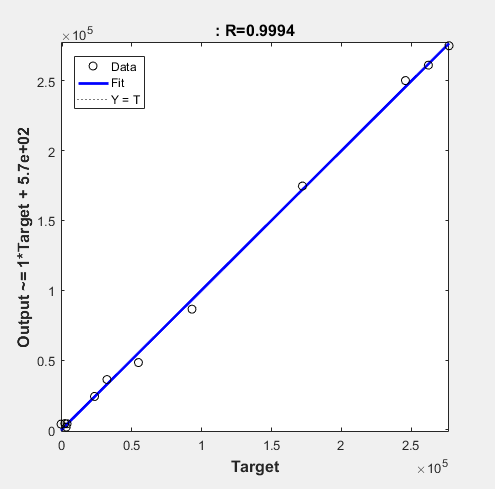
\includegraphics[width=.5\textwidth]{TIM20180704170021.png} %1.png是图片文件的相对路径
  \caption{线性回归相关系数R} 
  \label{TIM20180704170021} 
\end{figure}

同时,借助EXCEL的回归分析,可以得到如表\ref{tab:addlabela1}-\ref{tab:addlabela2}的分析表格(原表)和图\ref{Residual Plot}-\ref{TIM20180704210336.png}的残差图、线性拟合图和正态概率图。
% Table generated by Excel2LaTeX from sheet 'Sheet2'
\begin{table}[htbp]
  \centering
  \caption{EXCEL线性回归分析表}
    \begin{tabular}{ccccccc}
    \hline
       & Coefficients & 标准误差 & t Stat & P-value & 下限 95.0\% & 上限 95.0\% \bigstrut\\
    \hline
    Intercept & -2474.7 & 5117.461 & -0.48358 & 0.649118 & -15629.6 & 10680.15 \bigstrut[t]\\
    X Variable 1 & 0.680384 & 0.385964 & 1.762817 & 0.138221 & -0.31177 & 1.672537 \\
    X Variable 2 & -3.84507 & 1.952174 & -1.96964 & 0.105973 & -8.8633 & 1.173152 \\
    X Variable 3 & 0.023847 & 0.075854 & 0.314376 & 0.76593 & -0.17114 & 0.218835 \\
    X Variable 4 & 46.25212 & 18.30964 & 2.526108 & 0.05278 & -0.8143 & 93.31854 \\
    X Variable 5 & 0.658808 & 1.921831 & 0.342803 & 0.745689 & -4.28141 & 5.599031 \\
    X Variable 6 & -7.86877 & 2.287389 & -3.44007 & 0.018434 & -13.7487 & -1.98885 \\
    X Variable 7 & -29.1862 & 5.969913 & -4.88889 & 0.004518 & -44.5324 & -13.8401 \bigstrut[b]\\
    \hline
    \end{tabular}%
  \label{tab:addlabela1}%
\end{table}%

\begin{table}[htbp]
  \centering
  \caption{回归统计}
    \begin{tabular}{cc}
    \hline
    Multiple R & 0.999455 \bigstrut[t]\\
    R Square & 0.998911 \\
    Adjusted R Square & 0.997386 \\
    标准误差 & 5598.424 \\
    观测值 & 13 \bigstrut[b]\\
    \hline
    \end{tabular}%
  \label{tab:addlabel}%
\end{table}%

\begin{table}[htbp]
  \centering
  \caption{方差分析}
    \begin{tabular}{cccccc}
    \hline
       & df & SS & MS & F  & Significance F \bigstrut\\
    \hline
    回归分析 & 7  & 1.44E+11 & 2.05E+10 & 655.0666 & 4.25E-07 \bigstrut[t]\\
    残差 & 5  & 1.57E+08 & 31342348 &    &  \\
    总计 & 12 & 1.44E+11 &    &    &  \bigstrut[b]\\
    \hline
    \end{tabular}%
  \label{tab:addlabel}%
\end{table}%

\begin{table}[htbp]
  \centering
  \caption{残差输出表}
    \begin{tabular}{cccc}
    \hline
    观测值 & 预测 Y & 残差 & 标准残差 \bigstrut\\
    \hline
    1  & 23832.86 & -630.611 & -0.1745 \bigstrut[t]\\
    2  & 36317.8 & -4235.51 & -1.17205 \\
    3  & 48392.23 & 6261.816 & 1.732767 \\
    4  & 86891.34 & 6110.138 & 1.690795 \\
    5  & 174426.2 & -2387.02 & -0.66054 \\
    6  & 275212.7 & 1760.826 & 0.487255 \\
    7  & 249575.4 & -3768.23 & -1.04274 \\
    8  & 261286.5 & 933.4399 & 0.258301 \\
    9  & 4172.994 & -4985.99 & -1.37972 \\
    10 & 1528.118 & 1350.882 & 0.373815 \\
    11 & 4096.499 & -2146.5 & -0.59398 \\
    12 & 4211.935 & -737.935 & -0.2042 \\
    13 & -2474.7 & 2474.7 & 0.684798 \bigstrut[b]\\
    \hline
    \end{tabular}%
  \label{tab:addlabel}%
\end{table}%

\begin{table}[htbp]
  \centering
  \caption{概率输出}
    \begin{tabular}{cc}
    \hline
    百分比排位 & Y \bigstrut\\
    \hline
    3.846154 & -813 \bigstrut[t]\\
    11.53846 & 0 \\
    19.23077 & 1950 \\
    26.92308 & 2879 \\
    34.61538 & 3474 \\
    42.30769 & 23202.25 \\
    50 & 32082.29 \\
    57.69231 & 54654.05 \\
    65.38462 & 93001.48 \\
    73.07692 & 172039.1 \\
    80.76923 & 245807.2 \\
    88.46154 & 262220 \\
    96.15385 & 276973.6 \bigstrut[b]\\
    \hline
    \end{tabular}%
  \label{tab:addlabela2}%
\end{table}%

\begin{figure}[htbp]
  \centering
  \begin{tabular}{cc}
  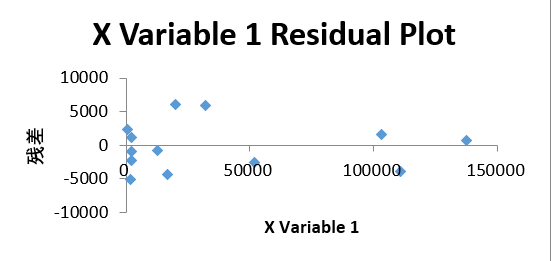
\includegraphics[width=.45\textwidth]{TIM20180704204332.png} & 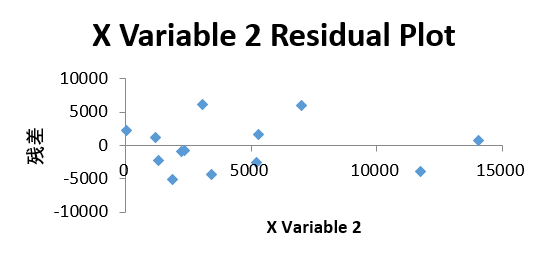
\includegraphics[width=.45\textwidth]{TIM20180704204923.png}\\
  $\alpha_1$&$\alpha_2$\\
  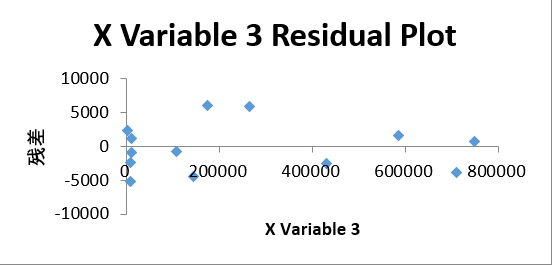
\includegraphics[width=.45\textwidth]{TIM20180704205304.png}&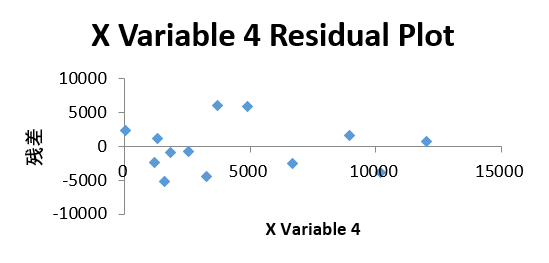
\includegraphics[width=.45\textwidth]{TIM20180704205341.png}\\
  $\alpha_3$&$\alpha_4$\\
    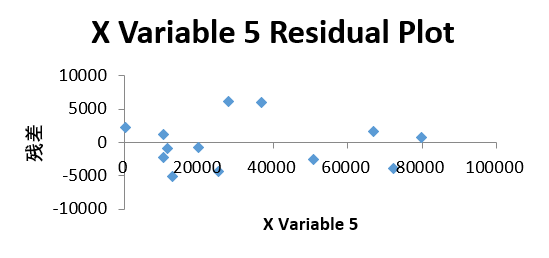
\includegraphics[width=.45\textwidth]{TIM20180704205413.png} & 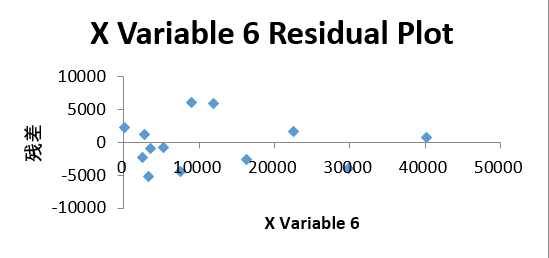
\includegraphics[width=.45\textwidth]{TIM20180704205443.png}\\
  $\alpha_5$&$\alpha_6$\\
  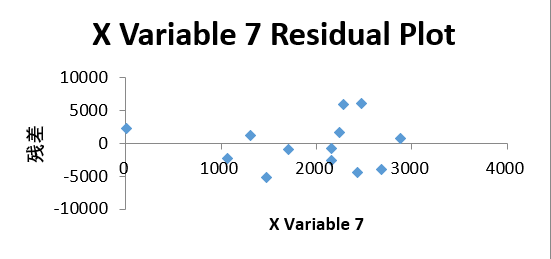
\includegraphics[width=.45\textwidth]{TIM20180704205513.png}&\ \\
  $\alpha_7$&\ 
  \end{tabular}
  \caption{残差图} 
  \label{Residual Plot} 
\end{figure}
\begin{figure}[htbp]
  \centering
  \begin{tabular}{cc}
  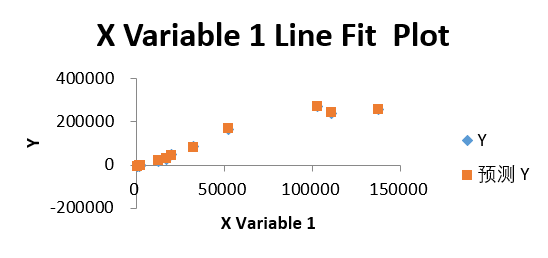
\includegraphics[width=.45\textwidth]{TIM20180704205802.png} & 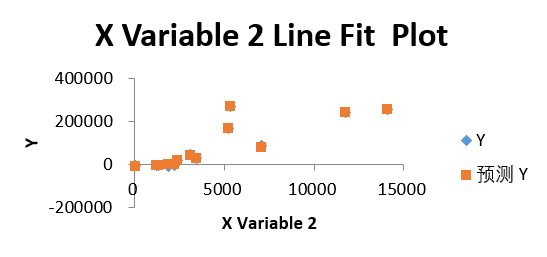
\includegraphics[width=.45\textwidth]{TIM20180704205833.png}\\
  $\alpha_1$&$\alpha_2$\\
  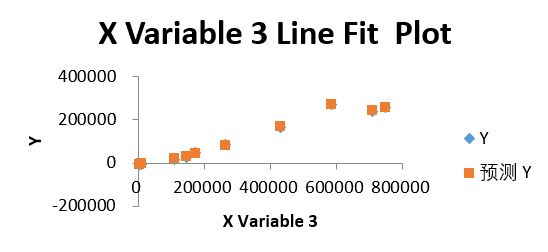
\includegraphics[width=.45\textwidth]{TIM20180704205915.png}&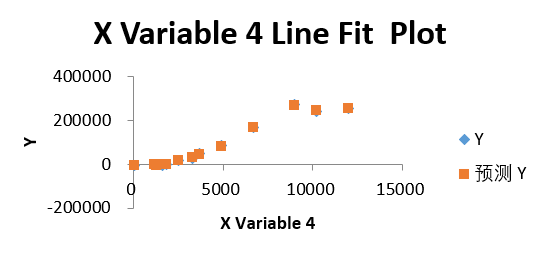
\includegraphics[width=.45\textwidth]{TIM20180704205938.png}\\
  $\alpha_3$&$\alpha_4$\\
    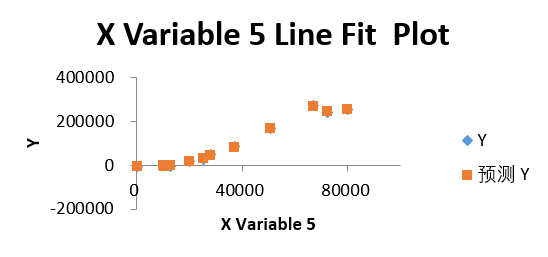
\includegraphics[width=.45\textwidth]{TIM20180704210023.png} & 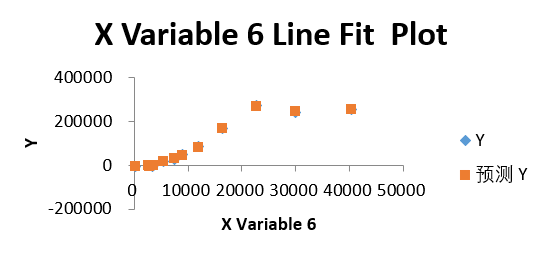
\includegraphics[width=.45\textwidth]{TIM20180704210058.png}\\
  $\alpha_5$&$\alpha_6$\\
  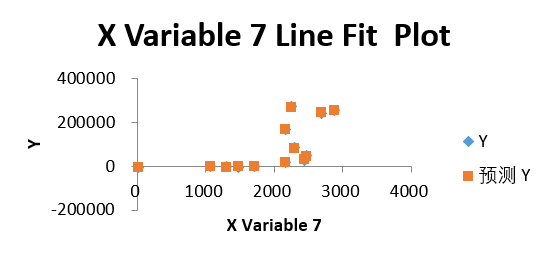
\includegraphics[width=.45\textwidth]{TIM20180704210136.png}&\ \\
  $\alpha_7$&\ 
  \end{tabular}
  \caption{线性拟合图} 
  \label{Line Fit  Plot} 
\end{figure}
\begin{figure}[htbp]
  \centering
  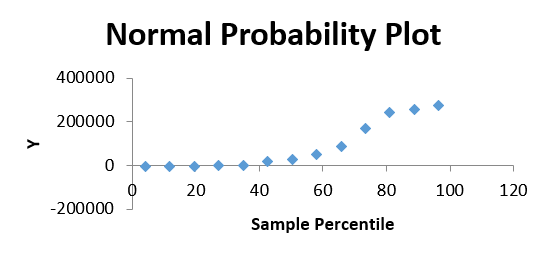
\includegraphics[width=.7\textwidth]{TIM20180704210336.png} 
  \caption{正态概率图} 
  \label{TIM20180704210336.png} 
\end{figure}

在表与图中可以看到,由EXCEL拟合的参数$X\ Variable\ i$也与$a_i$的值大致接近,由情况分析表与线性拟合图、正态概率图及相关系数R可知,作为线性拟合的多项式与原函数契合程度好,且由MATLAB生成的R图像可知,线性回归拟合并没有出现过拟合的现象,即由此模型得到的结果是十分可信的。

由此,我们得到利润函数为
\begin{equation}
y=0.6716x_1-3.9372x_2+0.0405x_3+46.5675x_4+0.4558x_5-7.8513x_6-29.5005x_7
\end{equation}
由该函数各项系数情况,我们可以得知,为做到利润最大化,在生产管理过程中,可以试着:
\begin{enumerate}[1.]\addtolength{\itemsep}{-1.5ex}
\item 在安全性上不要做过多的投入;
\item 适当削减在生产制造、研发方面的投入,注意控制成本;
\item 略微增加在生产设计、营销、维护方面的投入,注重客户前期需求的把握、中期宣传和售后服务;
\item 加大在测试上的投入,提高产品本身的质量。
\end{enumerate}
\subsection{模型二:考虑购买人群的管理优化模型}
\subsubsection{模型的准备}
将购买人群也纳入考虑,则首先要先知道实际购买(使用)人群分布情况。由于具体的职业划分难以十分具体,这里以年龄作为分组依据。通过调查,可以得到购买诺基亚8110的顾客分布情况大致如表\ref{tab:addlabelren1}所示。
\begin{table}[htbp]
  \centering
  \caption{购买诺基亚8110的年龄分布情况}
    \begin{tabular}{cc}
    \hline
    年龄 & \multicolumn{1}{l}{比例} \\
    \hline
    15以下 & 9.42  \\
    15-25 & 21.01  \\
    25-35 & 5.80  \\
    35-45 & 31.16  \\
    45-60 & 20.29  \\
    60以上 & 12.32  \\
    \hline
    \end{tabular}%
  \label{tab:addlabelren1}%
\end{table}%

从中可以看出,诺基亚8110的购买群体较广,大致在青少年及老年群体人数较多。
\subsubsection{模型的建立与求解}
对于不同的对象,对产品会有不同的需求,这一需求表现在生产过程中就是对不同环节$x_i$的重视情况$K_i$,当这一人群占购买对象比例为$p_k$时,得到修正后的利润函数模型:
\begin{equation}
y=G(x_i)=\sum_{k=1}^Np_k\sum_{i=1}^7K_{i}\sum_{j=0}^n\beta_{ij}x_i^j
\end{equation}
其中$\beta_{ij}$是待求的参数。在求出利润函数后,为找到利润最大时的取值,需要进一步求解,分别对利润函数的各个环节投入求偏导,得到使$\frac{\partial G}{\partial x_i}=0$的$x_i$族$g_{j}=\{x_{ij}|\frac{\partial G}{\partial x_{ij}}=0\}$

借助Heesen矩阵的的正定性,可以判断该极值点为极大值还是极小值。当然,由于我们需要得到最大值,故也可以直接写成
\begin{equation}
y_{MAX}=MAX\{g_1,g_2,\dots,g_j,\dots,g_J\}
\end{equation}
其中J为g的个数。
这便是修正之后寻找利润最大的方法,与该最大值对应的$g_j$就成为管理生产的目标。
\newpage
\section{Nokia 8110香蕉机全面评估报告}
在如今竞争激烈的手机市场中,各价位的手机往往都有明确的市场和用户定位。但看惯了旗舰和时尚代表的争奇斗艳,在百元机领域,诺基亚8110,将会是一个不可忽视的存在。

复刻经典机型,诺基亚8110机身采用弧形波浪的时尚设计,2.4英寸QVGA彩色屏幕,键盘布局更加合理,简洁的设计也让手机看起来精致了许多。而作为主推的黄色机型,更是被昵称为“香蕉机”,颇受瞩目和追捧。

姣好的外观,也不乏优良的配置。诺基亚8110,200万像素后置摄像头的手机,支持双卡和LTE连接。4G手机,却能超长待机25天。内置地图、流行社交软件等应用,新版贪吃蛇,更会让人停不下来。更有丰富的应用在应用商店等待。

拥有极高的颜值和不俗的配置的诺基亚8110,其性价比却会让人惊讶的眼珠子掉出来!百元机范围内鲜有敌手,火爆程度几可预期。

作为诺基亚智能手机重返之作重要一棋,诺基亚8110不仅是重新占领市场份额的一步,公司收益的提高也成为8110任务之一。

根据相关调查研究,产品利润的获得与产品生产环节的投入有着一定的关系。诺基亚8110的生产环节与最合理的资金投入有着相似的方案。在产品的测试上,诺基亚8110加大投入,更加注重产品质量。而在营销和维护方面,我们将适当投入,获得更大的宣传效果。同时适当控制生产制造成本,争取更大的潜在收益。

总而言之,作为一款百元机,诺基亚8110在各个方面都能满足日常的使用需求。精致小巧的机身,配上2.4英寸QVGA彩色屏幕,外观方面已然十分优秀。以及有超长续航加持的加持,火爆是不用担心的问题。诺基亚8110,难以想象的前景,这样一款物超所值的产品,期待您的投资!
\newpage
\section{模型分析}
\subsection{假设的合理性分析}
\begin{enumerate}[1.]\addtolength{\itemsep}{-1.5ex}
\item 假设一确保了数据的可靠性;
\item 假设二排除了各要素间相互作用的影响,也简化了了最终利润与各环节投入间关系的计算,使模型更高效;
\item 假设三排除了偶然因素对最终结果的影响,使得对各个环节资金投入与利润间关系的研究有理论意义;
\item 假设四排除了无法量化的波动因素对结果的影响,使得模型可以得到相对确定的结果;
\item 假设五使模型更符合实际;
\end{enumerate}
\subsection{模型的合理性分析}
本文所提供的模型充分考虑到了各生产环节与利润的相互制约关系,通过合理的假设明确各环节之间的关系,通过查阅相对权威的期刊或文献,获得真实可靠的数据,即原始条件以及数据有合理性。

模型的建立过程中,运用泰勒定理,以多项式拟合利润函数,通过求利润函数的极值位置来确定利润最大值及对应的管理方案,同时用MATLAB和EXCEL等成熟的软件进行回归分析并进行回归的合理性分析、过拟合情况分析,体现了模型设计中算法过程以及求解过程的合理性。

最终的结果同时考虑了其他影响因子,并进行综合考量改进,即结果有合理性。
\section{模型的评价与优化}
\subsection{模型的优点}
\begin{enumerate}[1.]\addtolength{\itemsep}{-1.5ex}
\item 通过合理的假设,排除一些无关因素及不重要因素对模型的干扰,使得模型更稳定,计算结果更可靠;
\item 本文中的模型,通过多项式来拟合利润函数并求解其极值来得到最终解,得到的最终结果具有可靠度高,与实际结果符合程度好的优点;
\item 模型综合考虑了多种影响因子,计算结果的可信度高,符合实际情况。
\item 通过寻找极值来确定最大利润及对应的管理方案,事实上提供了找寻所有较大利润管理方案的方法,对于难以达到最大利润的情况,还可以求其次大,只需将最大值去除后在进行一次模型即可。
\end{enumerate}
\subsection{模型的缺点}
\begin{enumerate}[1.]\addtolength{\itemsep}{-1.5ex}
\item 由于假设中排除了一些偶然因素,在实际生产销售中,可能会有略微的差异;
\item 本模型事实上需要对最高次相关项进行判断,这一点虽然可以借助相应的软件快速完成,但对于变量非常多的情况,模型的效率可能并不高。
\end{enumerate}
\subsection{模型的优化}
\begin{enumerate}[1.]\addtolength{\itemsep}{-1.5ex}
\item 考虑到对市场的分析,以往利润与各生产环节投入间关系存在一定的时间联系,可以引入时间影响因子$T(t)$。
\item 考虑到实际生产、销售过程中可能存在的偶然因素,可以引入随机波动影响因子$Q$。
\end{enumerate}
\section{模型应用领域及推广}
本文提出的基于各生产环节投入的利润最大化模型、管理优化模型,无论是作为前期开发新产品的预算分配的计算参考,还是作为产品投放前的可能利润情况预判,都是极好的选择。

在学习一定量的,例如各个季度各生产环节资金投入与例如关系后,可以更为准确、及时地给出具体的方案,可以作为利润情况的预判分析,也可以在产品的投入分配规划等方面发挥一定作用。
\begin{thebibliography}{15}\zihao{5}\addtolength{\itemsep}{-2.5ex}\addcontentsline{toc}{section}{参考文献}
\bibitem{xu}许茂增,唐飞.考虑消费者偏好的闭环供应链差别定价模型[J].计算机集成制造系统,2014,20(04):945-954.
\bibitem{zhao}张旭梅,官子力,范乔凌,王大飞,但斌.考虑网络外部性的电信业产品服务供应链定价与协调策略[J].管理学报,2017,14(02):270-276.
\bibitem{weng}翁世淳,黄维.基于非合作博弈的智能手机定价策略研究[J].中国市场,2013(11):87-95.
\bibitem{pingguo}晁国喻.探讨商业模式与财务报表的关联性——以苹果公司为例[J].商,2015(18):133.
\bibitem{zhongxing} 解倩莹.中兴通讯公司财务报表分析与评价[J].中国管理信息化,2016,19(24):28-29.
\bibitem{xiaomi} 温艺晗. 小米携手美的 财务状况显山露水[N]. 中国联合商报,2014-12-22(E04).:14-17+50.
\bibitem{nuojiya} \url{https://www.nokia.com/en_int/about-nokia/investors/reports-and-filings}
\end{thebibliography}
%\renewcommand\appendicename{\heiti\zihao{5} 附录}.
\renewcommand\appendix{\setcounter{secnumdepth}{-2}}
\appendix
\titleformat{\section}{\centering\heiti\zihao{4}}{}{0.3em}{}
\section{附录}
\renewcommand\appendix{\setcounter{secnumdepth}{4}}
\renewcommand\thesubsection{\fontsize{12pt}{1}附录\arabic{subsection}}
\subsection{ MATLAB程序代码}
%\twocolumn
\begin{lstlisting}
data.txt
12159 	2296 	105207 	2482 	19665 	5190 	2144 	23202 
16293 	3378 	141589 	3232 	24961 	7360 	2422 	32082 
19605 	3020 	170453 	3637 	27536 	8847 	2456 	54654 
31644 	6975 	262426 	4838 	36615 	11827 	2276 	93001 
51614 	5150 	427616 	6650 	50433 	16121 	2144 	172039 
102552 	5250 	583016 	8907 	66633 	22439 	2230 	276974 
110151 	11707 	707523 	10154 	71877 	29700 	2675 	245807 
136877 	14010 	745034 	11966 	79595 	40093 	2867 	262220 
1429 	1799 	6347 	1550 	12485 	3130 	1468 	-813 
1839 	1144 	7295 	1256 	10150 	2550 	1293 	2879 
1600 	1243 	6097 	1144 	10052 	2382 	1051 	1950 
1931 	2158 	6874 	1774 	11256 	3359 	1697 	3474 

function main
clc
clear
data=load('data.txt');
y=data(:,8);
x=data(:,1:7);
beta=[1,0.05,0.02,0.1,0.1,0.1,0.1];            % first number 
yy=fun(beta,x);
[beta_out,r,J,COVB,mse]=nlinfit(x,y,@fun,beta);    
beta_out
mse
betaci=nlparci(beta_out,r,'Jacobian',J);   
betaa=[beta_out',betaci]     
[yy,delta]=nlpredci(@fun,x,beta_out,r,'Jacobian',J); 
alpha=0.05;
%nlintool(x,y,'fun',beta,alpha)  
r=corrcoef(y,yy)       % R
plotregression(y,yy)   
regstats(y,yy)

function yy=fun(beta,x)
b1 = beta(1);
b2 = beta(2);
b3 = beta(3);
b4 = beta(4);
b5 = beta(5);
b6 = beta(6);
b7 = beta(7);
yy=b1*(x(:,1))+b2*(x(:,2))+b3*(x(:,3))+b4*(x(:,4))+...
b5*(x(:,5))+b6*(x(:,6))+b7*(x(:,7));
\end{lstlisting}
\end{document}